
From the preceding chapter we arrived to a clear picture of the needed closures terms.
In this chapter we will focus on how to obtain the closures terms. 
In the first section we will investigate the current of Euler-Euler simulation to get a much clearer view of what closure we currently use.
Then we make an overview of the author how research the closures terms though DNS. 
Once the needs are clearly identified we expose our strategy and a glimpse of our first results.

\section{Intro/Current state of dispersed two phase flow  modeling}
\subsection{CFD-PBM coupling}
\begin{itemize}
    \item \citet{morel2010comparison} they perform Euler-Euler models coupled with PBM for bubbly flow columns. 
    They compare experiments with their results.
    \item \citet{sporleder2012population} they perform 1D Euler-Euler models coupled with PBM for bubbly flow columns and expose all closing terms for both models. 
    \item In his thesis \citet{gemello2018modelling} aimed to model industrial bubbles columns process. 
    He combined CFD-PBM / QMOM methods, and obtain accurate agreement on bubbles size distribution for bubbly flows.
    Their prediction are made for different coalescence kernels, and they predict the mean Sauter diameter (ratio between volume and surface of the particles). 
    Furthermore, they deduce that the best model for homogeneous flow regime is the film drainage model. 
    For heterogeneous flows the critical approach velocity seemed better.
    The CFD side is represented by turbulence models, and it is found that the size distribution isn't dependent on the model used. 
    The use of turbulence model with CFD-PBM coupling is However not representative of the reality. 
    A numerical feature called Stokes binding is used, together with a statistical Lagrangian approach. 
    \item \citet{alam2022cfd}
    \item \citet{wang1995simultaneous} study numerically the PBM equations for buoyancy driven setting of shperical DROPS suspension.
    They describe the closures terms used.  
\end{itemize}
\subsection{Turbulence modeling with PDF-PBE}
\begin{itemize}
    \item  \citet{salehi2017population} coupled Large Eddy simulation to PDF-PBM to predict the distribution shape and size of droplets in atomization turbulent flows. 
    The dispersed phase is here modeled with a Lagrangian approach, and the drag force use the mean velocity difference between the averaged continuous phase and the dispersed phase.
    In case were the particle response time is of the same order of the time scale of turbulence the real velocity is approximated thanks to a model. 
    The strategy of stokes binding is to represent one notional particle a particle size.
\end{itemize}




\subsection{Numerical studies aiming to close the terms}
\subsubsection{Rate of coalescence}
\begin{itemize}
    \item \citet{manga1995collective} IBM to study the interaction between two-three or four drops.
\end{itemize}
\subsubsection{Drag forces on isolated particles}
\begin{itemize}
    \item \citet{magnaudet1997forces}
\end{itemize}
\subsubsection{Pseudo-Turbulent Tensor}
\begin{itemize}
    \item \citet{esmaeeli2005direct} try to recover $\bm{u'u'}$ by direct numerical simulations. 
    They consider only bubbly flows at Re = 100. 
    They also study dissipation and distribution functions.
    \item \citet{du2022analysis} perform a decomposition of the particles agitations. 
\end{itemize}
\paragraph{closing the terms though waves analisys}
\begin{itemize}
\subsubsection*{closing the terms though waves analisys}
    \item \cite{duru2002constitutive}
    \item \citet{willen2017continuity}
    \item \citet{derksen2007direct}
\end{itemize}
\subsubsection{Sedimentation of numerous drops in a large container}
This is the first configuration, it will allow us to study polydisperse  drops suspension.  
\begin{itemize}
    \item \citet{davis1985sedimentation} Study the physics of the Sedimentation processes of polydisperse suspension of particles. They found different region with a given size distribution for each region.
    \item DNS/VOF of 3D rising bubbles \citet{innocenti2020direct} on basilisk. 
    The investigation is focus on the turbulence induced by the particles. 
    In the first place a validation study is set to get correct numerical parameters, they conclude that the viscosity, and density ratio have to be realistic $\rho_f/\rho_b>100$ and $\mu_f/\mu_b \approx 100$(for bubbles at least).  
    Then in a second part they analyze velocity fluctuation and energy spectra and found a global $k ^{-3}$ scaling in 2D. At scales larger than one diameter we recover Kolmogorov scaling $E(k) \sim k^{2/3}$.   
    In 3D they still find the $k^{-3}$ scaling from the two-point statistics, but no Kolmogorov length scale appear. Interestingly they validate Large Eddy simulation (20-30 point pre diameter) to analyze large scale properties. 
\end{itemize}

\subsubsection{Direct numerical simulation of Representative Elementary Volume}
\begin{itemize}
    \item Sedimentation of a suspension of rigid spheres \citet{willen2019resolved}
    \item DNS of periodic bubbly homogeneous flow \citet{tryggvason2006direct}
\end{itemize}

\subsubsection{Direct Numerical simulation}
In order to model film drainage in simulation one has to model all the different length scale from one diameter to $10^{-5}$ diameter. 
This is technically impossible in a suspension of drops.
Thus, several technics are available. 
\begin{itemize}
    \item \citet{thomas2010multiscale} implement theoretically the expression of the flow between the interface of the drop and a wall to avoid refining and solving the layer with DNS.
     This method enable us to the thinning of the film thinner than the length of a cell. 
\end{itemize}


\section{Basilisk a suited software to carry out massive DNS calculations }
All the numerical method (almost) are summarized in this book \citet{tryggvason2011direct}.

The VOF method is the method used to model two-phase flow. 
\begin{itemize}
    \item \citet{gueyffier1999volume} 
    \item \citet{popinet2009accurate} 
\end{itemize}
The level set Method :
\begin{itemize}
    \item \citet{osher2001level}
\end{itemize}

Lagrangian solver for multilayer solvers :
\begin{itemize}
    \item \citet{popinet2020vertically}
\end{itemize}

INCLUDE THE OTHER BIBLIO FROM THE BASILISK WEB SITE

\section{Obtaining closures terms with DNS}
\subsection{Numerical methods}

Scheme of the numerical domain
multigrid 

Navier-Stokes centered 

2D/3D

two-phase

tension

relative acceleration $\bm{a} = - \left[1-\frac{\left<\rho\right>}{\rho}\right]\bm{g}$

VALIDATION

no-coalescence

The range of study is presented \ref{tab:dim}. 
All the study had been performed on a sample of 100 droplets. 

Explain the link between the averaged variables in theory Vs in practice
\begin{table}[h!]
    \centering
    \begin{tabular}{||c|c|c|c||}
        \hline$Ga$&$Bo$&$\phi$&$\mu_f/\mu_d$\\ \hline
        $[0.1,100]$&$[0.1;1]$&$[0.05,0.25]$&$[0.042,0.42]$\\ \hline
    \end{tabular}
    \caption{dimensionless parameters investigated}
    \label{tab:dim}
\end{table}

 


\subsection{First results in 2 dimensional space}

\subsubsection{Drag force term}
The relative vertical velocity of the droplets with respect to the mean fluid motion, referred as $U$, it becomes constant.
Besides, we know that all the droplets experience a force of magnitude $\bm{F} = \phi Ls^2 \Delta \rho \bm{g}$, where $Ls$ is the domain size.
Thus, the averaged drag force per droplets is simply :
\begin{equation}
    \frac{\bm{f}}{\mu_f UD} = \left<V_b\right>\frac{\bm{g}\Delta \rho }{\mu_f D U}
    \label{eq:avgF}
\end{equation}  
where, $V_b$ is the averaged volume of droplets. 
We recall that the following results are carried out for a uniform distribution of bubbles thus $V_b = \left<V_b\right>$.
Besides, \ref{eq:avgF} is non-zero only on the vertical axis since $\bm{g} = g \bm{e}_y$. 
The drift velocity is computed by averaging the relative velocity on the time range where it is statistically stable.
This time range goes from $t = t_{min}$ to $t = t_{max}$, where the value of the dimensionless times are $t_{min} = 250$ and $t_{end} = 1000$. 
Thus, if we note $\left<\bm{u}\right>^d(t)$ the instantaneous velocity of the dispersed phase and $\left<\bm{u}\right>^f(t)$ the velocity of the fluid phase,
\begin{equation}
    \bm{U} =\left(t_{min}-t_{end}\right)^{-1}\int_{t_{min}}^{t_{end}}\left[\left<\bm{u}\right>^d(t)-\left<\bm{u}\right>^f(t)\right] dt.
\end{equation}

On the left graphic, \ref{fig:avgF}, we can note that the \textit{Bond number} has no influence on the mean drift velocity $\bm{U}$ for the set of parameters considered.
Indeed, as said in introduction, we are interested in very low \textit{Bond number} (see \ref{tab:parameters}).
Since there is no variation in the range $Bo = [0.1,1]$, we can consider that the system has reached its asymptotic behavior at $Bo<1$.
Furthermore, we also noted almost no variation with $Bo$ for all the other sets of parameters \ref{tab:dim}.
Consequently, the \textit{Bond number} dependency won't be considered in the present section. 
\begin{figure}[h!]
    \centering
    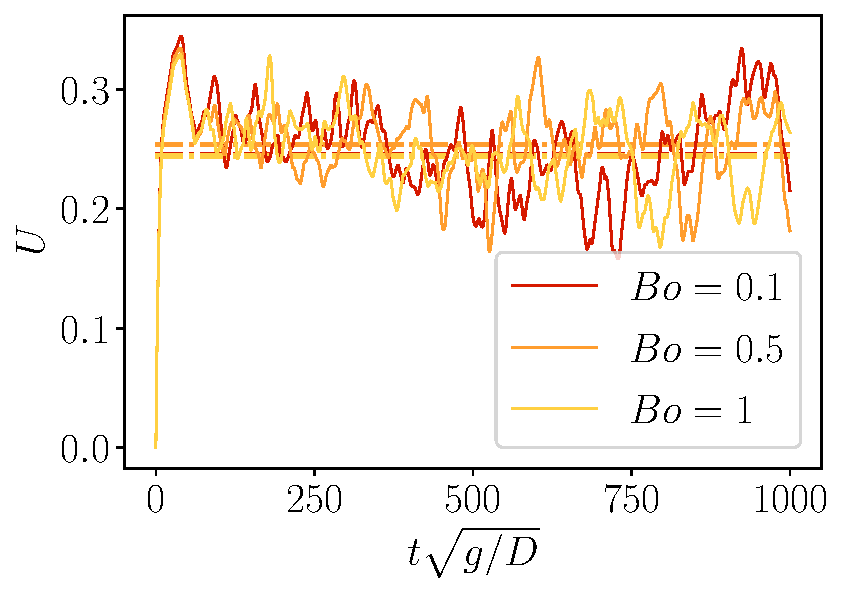
\includegraphics[height=0.22\textheight]{image/N_10/Favg/Bosdep_Ga_50.pdf}
    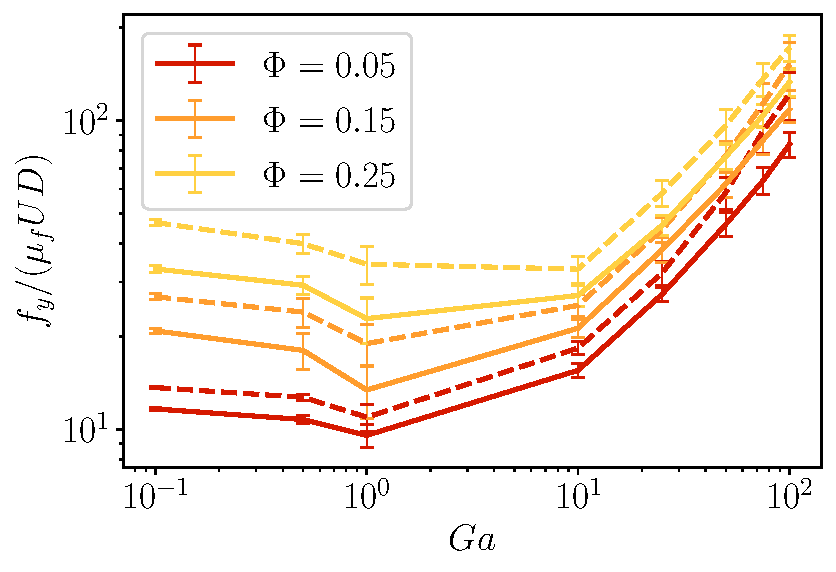
\includegraphics[height=0.22\textheight]{image/N_10/Favg/F_mu_Bo_0_5.pdf}
    \caption{(left) : Relative velocity in terms of the dimensionless time for different $Bo$ for $\phi = 0.15$, $\mu_r = 0.042$ and $Ga = 50$. (right) : Averaged drag force per droplets. Dashed lines : $\mu_f = 0.42$, solid lines : $\mu_f = 0.042$. The results are shown for $Bo = 0.5$.} 
    \label{fig:avgF}
\end{figure}
On the left graphic of \ref{fig:avgF} we can observe that for some studies at $Ga\le 1$, the dimensionless force is independent of the  \textit{Galileo number}. 
Besides, the averaged drag force increase with the volume fraction of droplets $\phi$.
While it decreases with increasing $\mu_r$. 

In the objective of designing the empirical formula describing the averaged force, we consider two steps. 
In the first place we consider a function, $g(\phi,\mu_r)$, independent of $Ga$ and $Bo$, which is asymptotic to $\bm{f}$ in the law $Ga$.
Then, the averaged force must be expressed by, $\bm{f} = \bm{g} \left[g(\phi,\mu_r) + f(\phi,\mu_r,Ga)\right]$ with $f(\phi,\mu_r,Ga)$ vanishing for small $Ga$. 
Besides, for $\phi \rightarrow 0$, the averaged force must tend to the isolated case scenario noted $\bm{f}_i(\mu_r)$. 
When $\phi \rightarrow 1$ the drag force must tend to infinity since no fluid goes through. 
Similarly, at $\mu_r \rightarrow \infty$, $\bm{f}_i$ must tend to the rigid spheres drag forces case,
at $Ga \rightarrow 0$ this force is comparable to the stokes drag force, referred as $\bm{f}_s$ \citep{guazzelli2011} ($\bm{f}_s/(\mu_r U D) = 3\pi$ for spheres, and \cite{khayat1989inertia}). 
And, when $\mu_r \rightarrow 0$ we should recover the drag force on rising bubbles from \citet{tomiyama1998drag}, we will note this force $\bm{f}_b$. 
Therefore, the function $g$ must respect the following composition,
\begin{equation}
    g(\phi,\mu_r) = \frac{C_1}{\phi - 1} + (\bm{f_i} - \bm{f_b}) e^{-\mu_r} + \bm{f_b}
\end{equation}
As one can observe on \ref{fig:avgF} the dependency with $Ga$, when $Ga>10$, behave as a power law. 
Therefore, 
\begin{equation}
    f(\phi,\mu_r,Ga) = C_1 Ga^{C_2}
\end{equation}

\subsubsection{Pseudo turbulence}
In the averaged equations for fluid and particulate phase seen \ref{chap:avg} need two-Pseudo turbulent tensor correlation,
namely, $\left<\bm{u'u'}\right>^p$ and $\left<\bm{u'u'}\right>^f$. 
Those tensors can be calculated as it is in the CFD code, since it is only fields variable average. 
Also, since our domain is homogeneous the crossed terms should be equal to 0.
Let's start by evaluating the fluid-phase average velocity fluctuations.
First note, that in the averaged equations, the important term isn't the pseudo-turbulent tensor itself but its divergence, namely,
\begin{equation*}    
    \left(\bm{\nabla} \cdot \left<\bm{u}'\bm{u}'\right>^f \right)_j = \frac{\partial <u_i' u_j'>^f}{\partial x_i}
\end{equation*}
where we make use of Einstein summation notation.
If the diagonal components are indeed null, it yields,
\begin{equation*}    
    \left(\bm{\nabla} \cdot \left<\bm{u}'\bm{u}'\right>^f \right)_j = \frac{\partial <u_j' u_j'>^f}{\partial x_j}
\end{equation*}
\begin{figure}[h!]
    \centering
    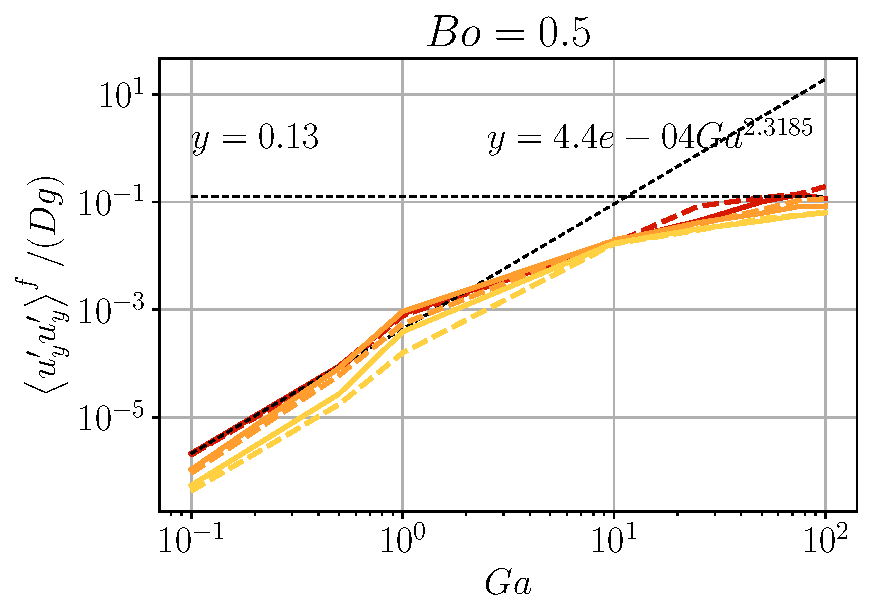
\includegraphics[height=0.22\textheight]{image/N_10/UU/UU_fyy_Bo_0_5.pdf}
    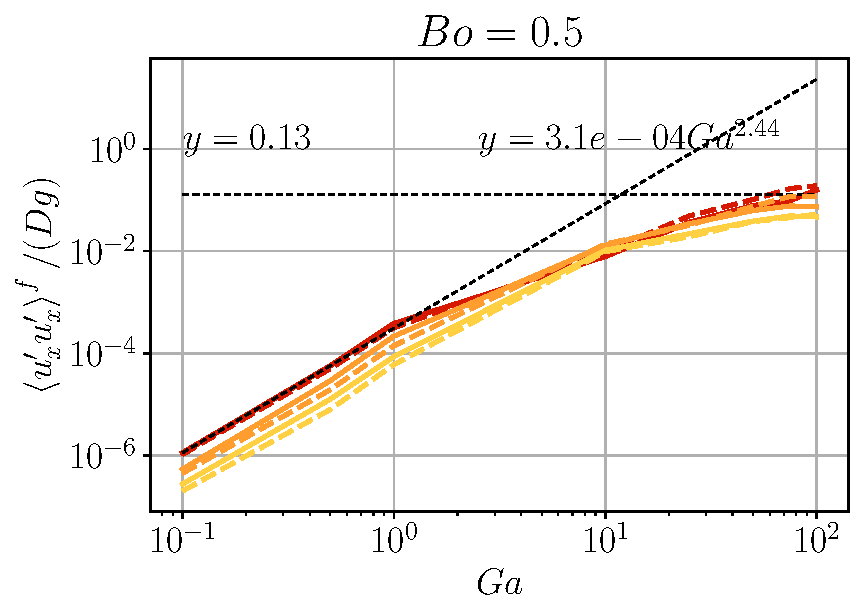
\includegraphics[height=0.22\textheight]{image/N_10/UU/UU_fxx_Bo_0_5.pdf}
    \caption{Fluid-phase average of the dimensionless velocity fluctuations. Dashed lines : $\mu_f = 0.42$, solid lines : $\mu_f = 0.042$, Dotted lines : asymptotic fit for $\phi = 0.05$ and $\mu_r = 0.42$. The results are shown for $Bo = 0.5$.} 
    \label{fig:UUf}
\end{figure} 
On \ref{fig:UUf} we can observe that the diagonal of the pseudo-turbulent tensor $\left<\bm{u'u'}\right>^f$ weakly dependent on $\mu_r$ nor on $\phi$.
Regarding the dependency of  with $Ga$, we note a power law behavior when, $Ga \rightarrow 0$. 
We can note that $\left<{u_x'u_x'}\right>^f  < \left<{u_y'u_y'}\right>^f$.
Indeed, the fluctuation in the $\bm{e}_y$ direction are more important due to the gravity along this axis.  

\ref{fig:UUp} shows the particulate-phase average exhibit the same behavior as the fluid phase average. 
Nevertheless, the $x$ and $y$ fluctuation have the same value.
\begin{figure}[h!]
    \centering
    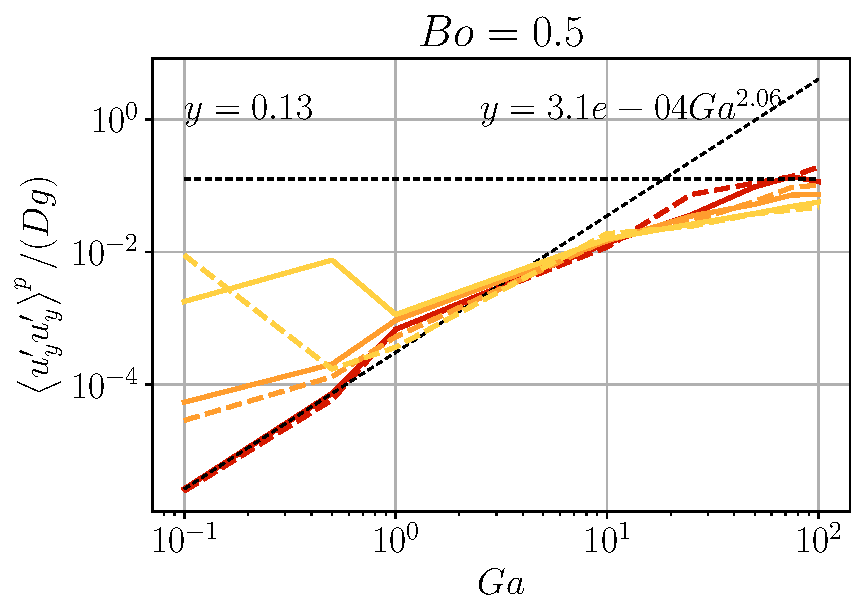
\includegraphics[height=0.22\textheight]{image/N_10/UU/UU_pyy_Bo_0_5.pdf}
    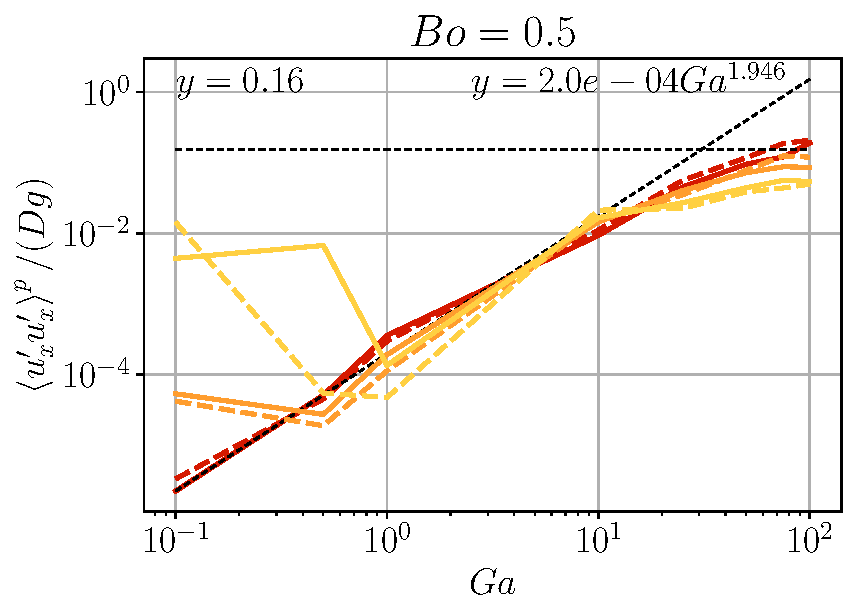
\includegraphics[height=0.22\textheight]{image/N_10/UU/UU_pxx_Bo_0_5.pdf}
    \caption{Fluid-phase average of the dimensionless velocity fluctuations. Dashed lines : $\mu_f = 0.42$, solid lines : $\mu_f = 0.042$, Dotted lines : asymptotic fit for $\phi = 0.05$ and $\mu_r = 0.42$. The results are shown for $Bo = 0.5$.} 
    \label{fig:UUp}
\end{figure} 

To estimate the value of the divergence of this tensor we consider a pipe flow where droplets are rising due to the gravity. 
Let's take a point far from a wall in our macroscopic medium. 
There, the Galileo number could be $Ga = 100$.
At the wall there are no velocities thus, the pseudo turbulent tensor and the velocities are both null.   
Therefore, 
\begin{equation*}    
    \left(\bm{\nabla} \cdot \left<\bm{u}'\bm{u}'\right>^f \right)_j = \frac{<u_j' u_j'>^f}{D}
\end{equation*}
In our case the scaling gives us a maximum of $10^{-2}$. 
If we compare this results to the drag force terms seen in the previous section we get an order of magnitude of two decades.
Therefore, this closure term has its importance, Nevertheless it might be negligible at this range of $Ga$. 

\subsubsection{The coalescence kernel}
\subsubsection{Collision behavior}
\subsubsection{Poly disperse simulations}

\subsubsection*{The 3 dimensional space simulations} 
It is working but it takes some time.
\subsubsection{Remarks and discussions}